%
\section{Introduction}

\begin{frame}{Who am I?}
  Marcus Müller
  \begin{itemize}
  \item started using \GR roughly 2010
  \item hung out too much on \texttt{discuss-gnuradio@gnu.org} and
    \texttt{usrp-users@lists.ettus.com}
  \item now does support work for Ettus
  \item while teaching and researching at the Karlsruhe Institute of
    Technology (KIT) / Communications Engineering Lab (CEL)
  \item Email: marcus@hostalia.de\\Twitter: @dEnergy\_dTime
  \end{itemize}
\end{frame}
\begin{frame}{What drives me mad}
  I often face problems like
  
  \begin{center}
    {\textit{I'm getting a lot of Overflows/Underflows! \GR sucks!}}
  \end{center}
\end{frame}
\section*{Overview}

\begin{frame}{Overview}
  \tableofcontents

\end{frame}

\section{Problem Statement}
\begin{frame}{Problem Statement}

  \begin{itemize}
  \item \GR is a sample pressure driven, pipelining architecture
  \item ``Just as slow
    as weakest link''
  \item When processing live signals, that must be faster than
    $f_\text{sample}$ of hardware.
  \end{itemize}
\end{frame}

\begin{frame}{Why is \GR especially hard?}
  \GR is running each block in its own thread,\\
  calling the \texttt{work} method as soon as

  \begin{itemize}
  \item new input items or
  \item additional output buffer space 
  \end{itemize}
  have become available.\\
  \bigskip
  simple matlab-style \texttt{tic}/\texttt{toc} won't cut it, here
\end{frame}

\begin{frame}{Flow Graph Under Test}
  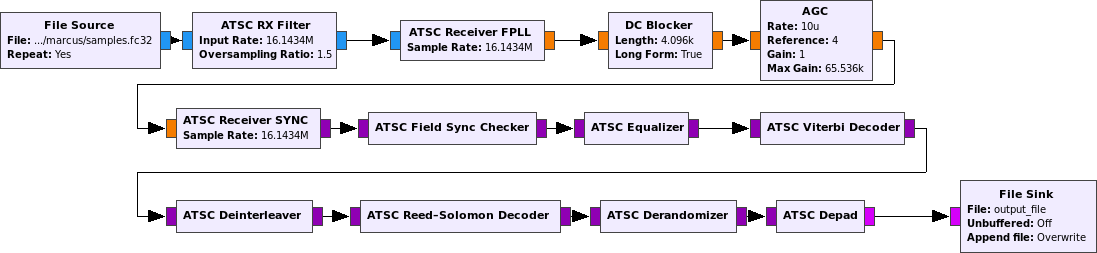
\includegraphics[width=\textwidth]{flowgraph}
\end{frame}

\section{Tools of Analysis}
\begin{frame}{Tools of Runtime Analysis}

  \begin{itemize}
  \item<1-2> \GR \textsc{Probe Rate}
  \item<1-2> Unix \texttt{top} / \texttt{htop}
  \item<1-2> Linux \texttt{perf}
  \item<1> \GR \textsc{ControlPort}
  \item<2> (\GR \textsc{ControlPort})
  \end{itemize}

\end{frame}
\begin{frame}{Probe Rate}
  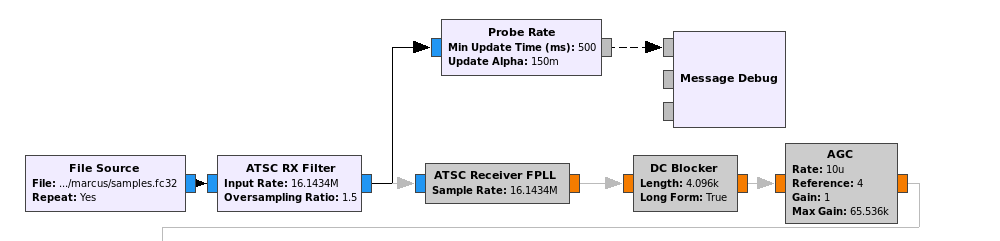
\includegraphics[width=\textwidth]{proberate}
\end{frame}
\begin{frame}{\texttt{htop}}
  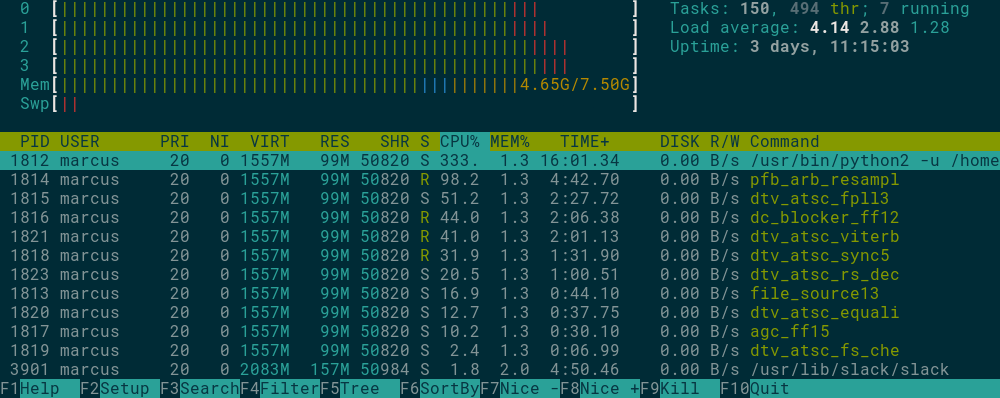
\includegraphics[width=\textwidth]{htop}
\end{frame}
\begin{frame}{\texttt{perf}}
  \begin{itemize}
    \item \texttt{perf}: Kernel-aided sampling of ``Where is my CPU right now?''
  \item Subcommands:
    \begin{itemize}
    \item \texttt{perf top}: Do a live sampling/display
    \item \texttt{perf record}: Execute and record the samples
    \item \texttt{perf report}: Display a previously recorded measurement
    \end{itemize}
  \item Caveat: You're sniffing around in what other processes do, that's
    against process segmentation
    \begin{itemize}
    \item \texttt{sudo sysctl kernel.perf\_event\_paranoid=-1} allows you to do
      that
    \item but also for everyone to probe how much time is spent in e.g.
        OpenSSL routines, so you \textit{might not want to} run this on your
        production system
    \end{itemize}
  \end{itemize}
\end{frame}
\section{The Usual Suspects}
\begin{frame}{The usual suspects}
  \begin{itemize}
  \item Convolution-based Bottleneck
    \begin{itemize}
    \item Filters
    \item Resamplers
    \item PLLs
      \item Correlators
    \end{itemize}
  \item Channel Decoders
  \end{itemize}
\end{frame}
\section{So, what do I do?}
\begin{frame}{So, what do I do?}
  \begin{itemize}
  \item Pick reasonable sample rates
    \begin{itemize}
    \item don't sample a 100\,kHz signal with 50 MS/s
    \end{itemize}
  \item Do reasonable filter design
  \item Resample reasonably
  \end{itemize}
\end{frame}

\begin{frame}{Do Reasonable Filter Design}
  \begin{itemize}
    \item Convolution: You need one multiplication + summation per filter tap
      per sample
    \item Number of taps in a filter:
      \begin{itemize}
    \item Formula I use\footnote{Taking this from  Bellanger's \textit{Digital Processing of Signals – Theory and Practice}; $\delta_1$: passband ripple, $\delta_2$:
        suppression, $\frac{f_s}{\Delta f}$: relation of sample rate to
        transition width}: $N\approx \frac 23 \log_{10} \left( \frac1{10
          \delta_1\delta_2}\right)\,\frac{f_s}{\Delta f}$
    \item There's a simpler formula (attributed to harris):
      $N\approx\frac{\delta_2}{22\frac{\Delta f}{f_s}}$
      \end{itemize}
    \item No, your filter does \textbf{not} need a stop-band attenuation of
      -100 dB.\\That's not even necessarily in the numerical dynamic of your
      numbers!
    \item No, your filter does \textbf{not} need a $\frac1{10000}$
      relative transition width!
    \item Not really design, but:
      \begin{itemize}
      \item If your filter isn't \textit{short}, fast convolution (\GR's
        \textsc{FFT Filter}) is your friend
      \end{itemize}
    \end{itemize}
\end{frame}
\begin{frame}{Resample reasonably}
    \begin{itemize}
    \item Integer decimators, interpolators, rational rate resamplers:
      \begin{itemize}
      \item Anti-Alias / Anti-Image filter
      \end{itemize}
    \item Arbitrary Resamplers
      \begin{itemize}
      \item Typically clever interpolators
        \item number and/or length of fractionally delaying filters to ``pick''
          the closest version
        \item the more, the less jitter
        \item the longer, the less aliasing artifacts
        \end{itemize}
        \item if after canceling all common factors, $1\gg\frac{r_\text{out}}{r_\text{in}}\in \mathbb Q$ and fixed, go for rational
          resampling!
    \end{itemize}
\end{frame}
\section{Conclusion}

\begin{frame}{Wrapping things up}
  \begin{itemize}
  \item \GR can be hard to analyze run-time wise (see simpleXecutive's talks)
  \item Not all is lost, because
    \begin{itemize}
    \item \texttt{(h)top} lets you have a look at \textit{who} uses your CPU
    \item \texttt{perf} tells you \textit{where} the CPU spends its time
      \item \textsc{Probe Rate} and other \GR tools help you look into the
        runtime behaviour
      \end{itemize}
    \item Common Pitfalls to be avoided
      \begin{itemize}
      \item overspecified filters
      \item crazy resamplers
        \item generally, bad design
      \end{itemize}
  \end{itemize}
\end{frame}